\documentclass[
	article,
	12pt,
	openright,
	oneside,
	a4paper,
	english,
	french,
	spanish,
	brazil
	]{abntex2}

\usepackage{lmodern}
\usepackage[T1]{fontenc}
\usepackage[utf8]{inputenc}
\usepackage{indentfirst}
\usepackage{color}
\usepackage{graphicx}
\usepackage{microtype}
\usepackage{filecontents}
\usepackage{listings}\usepackage{multirow}\usepackage{caption}\usepackage{amssymb}\usepackage{subcaption}\usepackage{tikz}\usetikzlibrary{automata, arrows}\tikzset{every picture/.style={line width=0.75pt}}

\usepackage[brazilian,hyperpageref]{backref}
\usepackage[alf]{abntex2cite}

% --- 
% CONFIGURAÇÕES DE PACOTES
% --- 

\renewcommand{\backrefpagesname}{Citado na(s) página(s):~}
\renewcommand{\backref}{}
\renewcommand*{\backrefalt}[4]{
	\ifcase #1 %
		Nenhuma citação no texto.%
	\or
		Citado na página #2.%
	\else
		Citado #1 vezes nas páginas #2.%
	\fi}%

\titulo{Detecção de vértices e arestas de cortes em grafos}
\autor{Lorhan Sohaky}
\data{26/11/2019}
\begin{filecontents}{bibliography.bib}
@misc{cormen,author="Thomas H. Cormen and Charles E. Leiserson and Ronald L. Rivest and Clifford Stein",title="Algoritmos",year="2002"}
@misc{italiano2012,author="Giuseppe F. Italiano and Luigi Laura and Federico Santaroni",title="Finding strong bridges and strong articulation points in linear time",year="2012"}
@misc{ibarra1993,author="Oscar H. Ibarra and Qi Zheng",title="Finding Articulation Points and Bridges of Permutation Graph",year="1993"}
@misc{madhumangal1998,author="Madhumangal AND Pal",title="Efficient Algorithms to compute all articulation points of a permutation graph",year="1988"}
@misc{henzinger2015,author="Monika Henzinger and Sebastian Krinninger and Veronika Loitzenbauer",title="Finding 2-edge and 2-vertex strongly connected components in quadratic time",year="2015"}
\end{filecontents}

\definecolor{blue}{RGB}{41,5,195}

\makeatletter
\hypersetup{
		pdftitle={\@title}, 
		pdfauthor={\@author},
    	pdfsubject={\imprimirpreambulo},
	    pdfcreator={LaTeX with abnTeX2},
		pdfkeywords={abnt}{latex}{abntex}{abntex2}{trabalho acadêmico}, 
		colorlinks=true,
    	linkcolor=blue,
    	citecolor=blue,
    	filecolor=magenta,
		urlcolor=blue,
		bookmarksdepth=4
}
\makeatother
% --- 

\makeatletter
\setlength{\@fptop}{5pt}
\makeatother
% ---

\newcommand{\quadroname}{Quadro}
\newcommand{\listofquadrosname}{Lista de quadros}

\newfloat[chapter]{quadro}{loq}{\quadroname}
\newlistof{listofquadros}{loq}{\listofquadrosname}
\newlistentry{quadro}{loq}{0}

\setfloatadjustment{quadro}{\centering}
\counterwithout{quadro}{chapter}
\renewcommand{\cftquadroname}{\quadroname\space} 
\renewcommand*{\cftquadroaftersnum}{\hfill--\hfill}

\setfloatlocations{quadro}{hbtp}
% ---

\setlength{\parindent}{1.3cm}

\setlength{\parskip}{0.2cm}

\makeindex

\begin{document}
\selectlanguage{brazil}
\frenchspacing
\imprimircapa
\imprimirfolhaderosto

\section{Resumo}
Este trabalho tem como objetivo apresentar um algoritmo para detectar arestas e vértices de cortes  a partir dos algoritmos de Busca em Largura e Busca em Profundidade em grafos não-dirigidos; e comparar o resultado obtido com outros algoritmos para verificar sua eficácia. A estratégia é  trabalhar sobre as árvores resultantes dos algoritmos de busca para chegar na solução.


\textbf{Palavras-chave}: vértice de corte, aresta de corte, busca em largura, busca em profundidade, grafo.

\section{Introdução}
A detecção de arestas e vértices de corte está presente em diversos problemas do cotidiano, mesmo que de forma imperceptível, são problemas como, por exemplo, detectar pontos de vulnerabilidade de uma rede de computadores, o impacto da perda de um dos pontos de distribuição de um produto / serviço e pontos frágeis de comunicação numa organização hierárquica. Verificar arestas e vértices de corte é importante para estipular a topologia do grafo ao remover uma aresta.

Teoria dos Grafos é um ramo da matemática que estuda a relação entre objetos de um determinado conjunto. Em que \textit{V} representa o conjunto de vértices e \textit{A} o conjunto de arestas do grafo \textit{G}. Representado por:

$G=(V,A)$

$A={(x,y) | x, y \in V}$

Uma aresta $a \in A$ de corte se \textit{G - a} é desconexo, ou seja, a remoção de uma aresta-de-corte desconecta o grafo. Um vértice \textit{v} é  considerado um vértice de corte se e somente se \textit{v} tem um filho \textit{t} tal que \(\nexists\) aresta ligando qualquer descendente de \textit{t} a um ancestral de \textit{v} \cite{cormen}.

Uma árvore é formada por um conjunto de elementos chamados nós. Toda a árvore possui um elemento chamado raiz, que está ligado a outros elementos chamados filhos ou ramos. Estes ramos podem estar ligados a outros elementos e assim sucessivamente. O elemento que não possui filhos é denominado como nó folha. A profundidade de um nó é a distância deste nó até a raiz da árvore. Um conjunto de nós com a mesma profundidade é chamado nível.

O algoritmo de busca em largura (\textit{Breadth-First Search - BFS} ) começa por um vértice raiz qualquer, e explora todos vértices que estão no mesmo nível, então avança para os vértices do nível seguinte e assim sucessivamente até que não haja mais vértices inexplorados, resultando em uma árvore com a ordem em que os vértices foram sendo explorados. Em resumo, a cada novo nível descoberto, todos os vértices daquele nível devem ser visitados antes de prosseguir para o próximo nível.

O algoritmo de busca em profundidade (\textit{Depth-First Search - DFS}) começa num vértice raiz qualquer, e explora um vértice filho tanto quanto possível - até chegar num nó folha; quando não for mais possível é feito o retrocesso para o nó do nível superior e um outro vértice filho é explorado e, assim por diante, até que não haja mais vértices não descobertos, resultando em uma árvore com a ordem em que os vértices foram descobertos. Em resumo, esse método imita a exploração de um labirinto, tentando ir o mais longe possível e quando não houver mais caminho, volta para o ponto onde teve de escolher um dos caminhos.

Devido ao funcionamento distinto do \textit{DFS} e do \textit{BFS}, as árvores resultantes podem ser diferentes e é nessa diferença em que este artigo explora uma maneira de trabalhar com as árvores para encontrar as arestas e vértices de corte. A Figura X evidencia a diferença entre as árvores geradas usando \textit{BFS} e \textit{DFS}.

Na seção de Desenvolvimento é apresentada solução que foi desenvolvida,  como foi verificada a eficácia do algoritmo e a linguagem escolhida para desenvolver; na seção de Trabalhos são apresentados os trabalhos providos da revisão sistemática e que estão relacionados com este artigo e na seção de Considerações são apresentadas as principais dificuldades e limitações da solução.

\begin{figure*}[htb]
    \caption{\label{fig:comparacaoBFSeDFS} Comparação entre a ordem em que os vértices são encontrados usando os algoritmos \textit{BFS} e \textit{DFS}. A numeração dos vértices indica ordem em que eles foram descobertos em cada um dos algoritmos.}
    
    \centering
    \begin{subfigure}{0.45\textwidth}
    \caption{\label{fig:grafoBFS}Na busca em largura os vértices são descobertos por níveis, quando não houver mais vértices no mesmo nível é feita a busca nos ramos seguintes.}1
    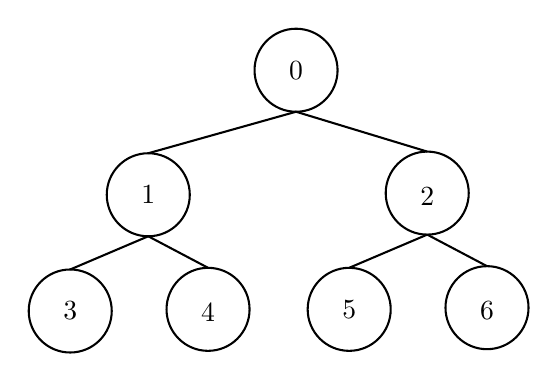
\begin{tikzpicture}[x=0.6pt,y=0.6pt,yscale=-1,xscale=1]
    \draw   (310,25) .. controls (310,11.19) and (321.19,0) .. (335,0) .. controls (348.81,0) and (360,11.19) .. (360,25) .. controls (360,38.81) and (348.81,50) .. (335,50) .. controls (321.19,50) and (310,38.81) .. (310,25) -- cycle ;
    \draw   (221,100) .. controls (221,86.19) and (232.19,75) .. (246,75) .. controls (259.81,75) and (271,86.19) .. (271,100) .. controls (271,113.81) and (259.81,125) .. (246,125) .. controls (232.19,125) and (221,113.81) .. (221,100) -- cycle ;
    \draw   (389,99) .. controls (389,85.19) and (400.19,74) .. (414,74) .. controls (427.81,74) and (439,85.19) .. (439,99) .. controls (439,112.81) and (427.81,124) .. (414,124) .. controls (400.19,124) and (389,112.81) .. (389,99) -- cycle ;
    \draw   (174,170) .. controls (174,156.19) and (185.19,145) .. (199,145) .. controls (212.81,145) and (224,156.19) .. (224,170) .. controls (224,183.81) and (212.81,195) .. (199,195) .. controls (185.19,195) and (174,183.81) .. (174,170) -- cycle ;
    \draw   (257,169) .. controls (257,155.19) and (268.19,144) .. (282,144) .. controls (295.81,144) and (307,155.19) .. (307,169) .. controls (307,182.81) and (295.81,194) .. (282,194) .. controls (268.19,194) and (257,182.81) .. (257,169) -- cycle ;
    \draw   (342,169) .. controls (342,155.19) and (353.19,144) .. (367,144) .. controls (380.81,144) and (392,155.19) .. (392,169) .. controls (392,182.81) and (380.81,194) .. (367,194) .. controls (353.19,194) and (342,182.81) .. (342,169) -- cycle ;
    \draw   (425,168) .. controls (425,154.19) and (436.19,143) .. (450,143) .. controls (463.81,143) and (475,154.19) .. (475,168) .. controls (475,181.81) and (463.81,193) .. (450,193) .. controls (436.19,193) and (425,181.81) .. (425,168) -- cycle ;
    \draw    (335,50) -- (246,75) ;
    \draw    (335,50) -- (414,74) ;
    \draw    (199,145) -- (246,125) ;
    \draw    (246,125) -- (282,144) ;
    \draw    (414,124) -- (367,144) ;
    \draw    (450,143) -- (414,124) ;
    \draw (335,25) node  [align=left] {0};
    \draw (246,100) node  [align=left] {1};
    \draw (414,101) node  [align=left] {2};
    \draw (199,170) node  [align=left] {3};
    \draw (282,171) node  [align=left] {4};
    \draw (367,169) node  [align=left] {5};
    \draw (450,170) node  [align=left] {6};
    \end{tikzpicture}
    \end{subfigure}
    ~
    \begin{subfigure}{0.45\textwidth}
    \caption{\label{fig:grafoDFS} Na busca em profundidade os ramos são explorados e quando não for mais houver mais ramos é feito retrocesso e os vértices vizinhos são explorados.}
    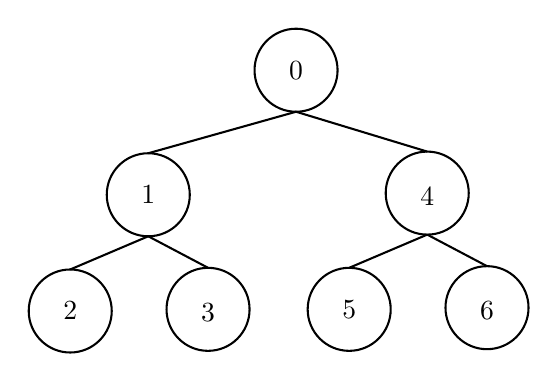
\begin{tikzpicture}[x=0.6pt,y=0.6pt,yscale=-1,xscale=1]
    \draw   (310,25) .. controls (310,11.19) and (321.19,0) .. (335,0) .. controls (348.81,0) and (360,11.19) .. (360,25) .. controls (360,38.81) and (348.81,50) .. (335,50) .. controls (321.19,50) and (310,38.81) .. (310,25) -- cycle ;
    \draw   (221,100) .. controls (221,86.19) and (232.19,75) .. (246,75) .. controls (259.81,75) and (271,86.19) .. (271,100) .. controls (271,113.81) and (259.81,125) .. (246,125) .. controls (232.19,125) and (221,113.81) .. (221,100) -- cycle ;
    \draw   (389,99) .. controls (389,85.19) and (400.19,74) .. (414,74) .. controls (427.81,74) and (439,85.19) .. (439,99) .. controls (439,112.81) and (427.81,124) .. (414,124) .. controls (400.19,124) and (389,112.81) .. (389,99) -- cycle ;
    \draw   (174,170) .. controls (174,156.19) and (185.19,145) .. (199,145) .. controls (212.81,145) and (224,156.19) .. (224,170) .. controls (224,183.81) and (212.81,195) .. (199,195) .. controls (185.19,195) and (174,183.81) .. (174,170) -- cycle ;
    \draw   (257,169) .. controls (257,155.19) and (268.19,144) .. (282,144) .. controls (295.81,144) and (307,155.19) .. (307,169) .. controls (307,182.81) and (295.81,194) .. (282,194) .. controls (268.19,194) and (257,182.81) .. (257,169) -- cycle ;
    \draw   (342,169) .. controls (342,155.19) and (353.19,144) .. (367,144) .. controls (380.81,144) and (392,155.19) .. (392,169) .. controls (392,182.81) and (380.81,194) .. (367,194) .. controls (353.19,194) and (342,182.81) .. (342,169) -- cycle ;
    \draw   (425,168) .. controls (425,154.19) and (436.19,143) .. (450,143) .. controls (463.81,143) and (475,154.19) .. (475,168) .. controls (475,181.81) and (463.81,193) .. (450,193) .. controls (436.19,193) and (425,181.81) .. (425,168) -- cycle ;
    \draw    (335,50) -- (246,75) ;
    \draw    (335,50) -- (414,74) ;
    \draw    (199,145) -- (246,125) ;
    \draw    (246,125) -- (282,144) ;
    \draw    (414,124) -- (367,144) ;
    \draw    (450,143) -- (414,124) ;
    \draw (335,25) node  [align=left] {0};
    \draw (246,100) node  [align=left] {1};
    \draw (414,101) node  [align=left] {4};
    \draw (199,170) node  [align=left] {2};
    \draw (282,171) node  [align=left] {3};
    \draw (367,169) node  [align=left] {5};
    \draw (450,170) node  [align=left] {6};
    \end{tikzpicture}
    \end{subfigure}
    \fonte{Próprio autor.}
\end{figure*}

\section{Desenvolvimento}
O algoritmo pode ser explicado em pseudo-código. Para solucionar o problema e poder testar com grafos maiores o algoritmo foi implementado na linguagem de programação Python, esta linguagem foi escolhida para tirar proveito de algumas bibliotecas já prontas para lidar com grafos, como por exemplo, a biblioteca \href{https://networkx.github.io/}{NetworkX}.

Foram gerados alguns grafos para testar o algoritmo de modo manual (no papel). Após testar o algoritmo em um conjunto de grafos, mais simples que podem ser facilmente desenhados no papel, o algoritmo foi submetido a um conjunto diferente de grafos para avaliar melhor sua eficácia. Os grafos escolhidos foram retirados do repositório de \citeonline{nr} e, são eles \href{http://networkrepository.com/aves-weaver-social-11.php}{aves-weaver-social-11}, \href{http://networkrepository.com/bn-fly-drosophila-medulla-1.php}{fly-drosophila-medulla-1}, \href{http://networkrepository.com/tech-WHOIS.php}{whois} e \href{http://networkrepository.com/web-webbase-2001.php}{webbase-2001}.

\subsection{Algoritmo}
O algoritmo, se baseia na diferença entre as árvores geradas pelo \textit{DFS} e \textit{BFS}. Visto que um vértice \textit{v} é considerado um vértice de corte se e somente se \textit{v} tem um filho \textit{t} tal que \(\nexists\) aresta ligando qualquer descendente de \textit{t} a um ancestral de \textit{v}, se na busca em largura aparecer um vértice filho de \textit{t} ligado a um ancestral de \textit{v}, isso caracteriza que \textit{v} não é um vértice de corte e, este filho de \textit{t} irá aparecer na árvore do \textit{BFS} devido a características de buscar por nível.

O algoritmo base em pseudo-código fica da seguinte maneira:

\begin{enumerate}
\item Gerar a árvore \textit{BFS} e \textit{DFS} a partir de um mesmo vértice \textit{a}, que será o primeiro ancestral em comum;
\item Para cada vértice $v \in DFS$ verificar se $\nexists (a,v)$ na \textit{BFS},  nesse caso o vértice \textit{w}, que é o ancestral de \textit{v} na \textit{DFS} passará a ser o novo ancestral em comum, a aresta \textit{(w,v)} passa a ser de corte e os vértices \textit{w} e \textit{v} são marcados como de corte.
\item Todo nó que for folha em ambas as árvores e tiver o mesmo ancestral em comum \textit{z}, este vértice \textit{z} é considerado vértice de corte.
\end{enumerate}

Algumas modificações foram necessárias pra trazer melhor corretude ao algoritmo, no passo 2, antes de considerar \textit{v} como de corte é verificado se este vértice é um nó folha, caso não seja, então pode ser considerado como de corte. Além disso, as arestas e vértices podem ser marcados como de corte mais de uma vez, então é necessário remover a repetição. O código Y é a implementação do algoritmo com as modificações citadas e uma verificação se o ancestral comum é diferente do vértice que está sendo analisado, isso serve apenas para melhorar a eficiência.

Implementação do algoritmo em Python.
\begin{lstlisting}[language=python]
import networkx as nx


def algoritmo(G, source):
	arestas_corte = []
	vertices_corte = []
	dfs_tree = nx.dfs_tree(G, source)
	bfs_tree = nx.bfs_tree(G, source)

	ancestral_comum = source
	for vertice in list(dfs_tree.nodes):
		if ancestral_comum != vertice and not (ancestral_comum,
				vertice) in list(bfs_tree.edges):
			predecessor = dict(nx.bfs_predecessors(dfs_tree,
							   source))[vertice]
			ancestral_comum = vertice

			arestas_corte.append((predecessor, vertice))
			vertices_corte.append(predecessor)
			if not (dfs_tree.out_degree(vertice) == 0
					and dfs_tree.in_degree(vertice) == 1
					and bfs_tree.out_degree(vertice) == 0
					and bfs_tree.in_degree(vertice) == 1
					and dict(nx.bfs_predecessors(dfs_tree,
					source))[vertice]
					== dict(nx.bfs_predecessors(bfs_tree,
					source))[vertice]):
				vertices_corte.append(vertice)
		elif dfs_tree.out_degree(vertice) == 0 \
			and dfs_tree.in_degree(vertice) == 1 \
			and bfs_tree.out_degree(vertice) == 0 \
			and bfs_tree.in_degree(vertice) == 1 \
			and dict(nx.bfs_predecessors(dfs_tree, source))[vertice] \
			== dict(nx.bfs_predecessors(bfs_tree, source))[vertice]:
			predecessor = dict(nx.bfs_predecessors(dfs_tree,
							   source))[vertice]
			vertices_corte.append(predecessor)

	return (vertices_corte, arestas_corte)
\end{lstlisting}

Para verificar a eficácia do algoritmo proposto, ele foi comparado com as funções \href{https://networkx.github.io/documentation/networkx-1.10/reference/generated/networkx.algorithms.components.biconnected.articulation_points.html}{articulation\_points} e \href{https://networkx.github.io/documentation/latest/reference/algorithms/generated/networkx.algorithms.bridges.bridges.html}{bridges} da biblioteca NetworkX.

O algoritmo proposto foi submetido ao caso de teste da figura W e a execução é demonstrada pela Tabela 1 . A figura Z mostra o segundo grafo de teste e sua execução na Tabela 2, é importante ressaltar que as arestas e vértices de corte em \textbf{negrito} são os falsos positivos.

\begin{figure*}[htb]
    \centering
    \begin{subfigure}{0.45\textwidth}
    \caption{Grafo do primeiro caso de testes.}
    \label{fig:caso-teste1}
    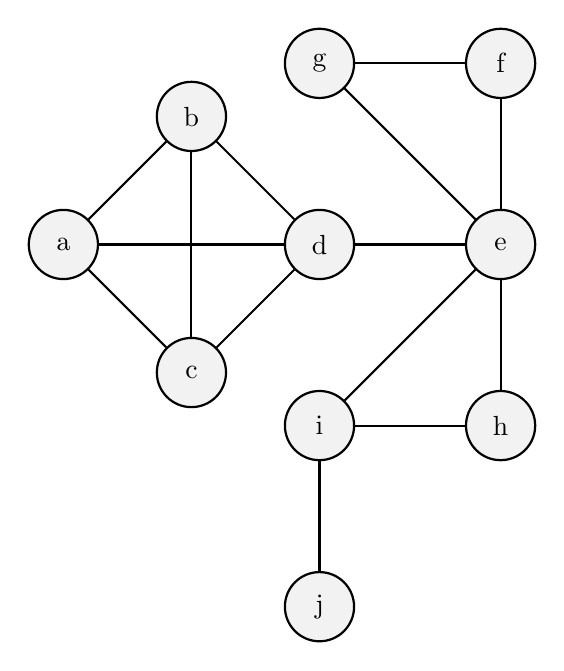
\begin{tikzpicture}[-,node distance=2.3cm,every state/.style={thick, fill=gray!10}, align=center]
        \node[state] (a) {a};
        \node[state,above right of=a] (b) {b};
        \node[state,below right of=b] (d) {d};
        \node[state,below right of=a] (c) {c};
        \node[state,right of=d] (e) {e};
        \node[state,above of=e] (f) {f};
        \node[state,left of=f] (g) {g};
        \node[state,below of=e] (h) {h};
        \node[state,left of=h] (i) {i};
        \node[state,below of=i] (j) {j};
        \draw
            (a) edge node{} (b)
            (a) edge node{} (d)
            (a) edge node{} (c)
            (b) edge node{} (d)
            (b) edge node{} (c)
            (c) edge node{} (d)
            (d) edge node{} (e)
            (e) edge node{} (g)
            (f) edge node{} (g)
            (e) edge node{} (f)
            (e) edge node{} (h)
            (e) edge node{} (i)
            (i) edge node{} (j)
            (i) edge node{} (h)
            ;
    \end{tikzpicture}
    \end{subfigure}
    ~
    \begin{subfigure}{0.45\textwidth}
    \caption{Grafo após aplicação do BFS. As arestas em destaque formam a árvore BFS. }
    \label{fig:caso-teste1-bfs}
    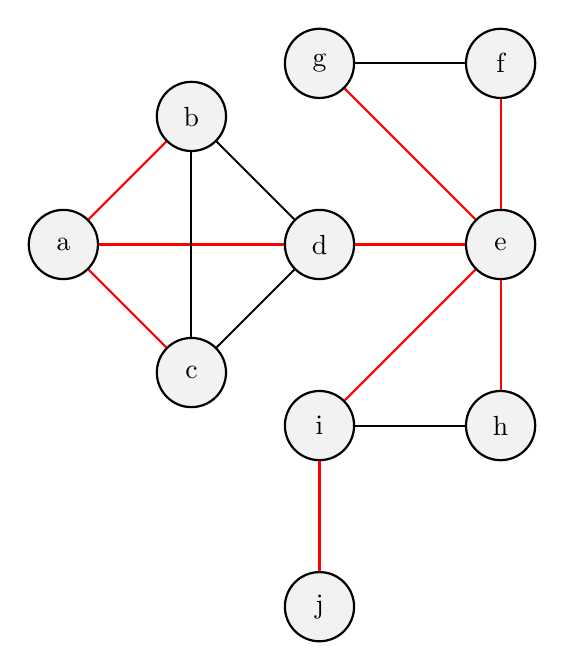
\begin{tikzpicture}[-,node distance=2.3cm,every state/.style={thick, fill=gray!10}, align=center]
        \node[state] (a) {a};
        \node[state,above right of=a] (b) {b};
        \node[state,below right of=b] (d) {d};
        \node[state,below right of=a] (c) {c};
        \node[state,right of=d] (e) {e};
        \node[state,above of=e] (f) {f};
        \node[state,left of=f] (g) {g};
        \node[state,below of=e] (h) {h};
        \node[state,left of=h] (i) {i};
        \node[state,below of=i] (j) {j};
        \draw
            (a) edge[color=red] node{} (b)
            (a) edge[color=red] node{} (d)
            (a) edge[color=red] node{} (c)
            (b) edge node{} (d)
            (b) edge node{} (c)
            (c) edge node{} (d)
            (d) edge[color=red] node{} (e)
            (e) edge[color=red] node{} (g)
            (f) edge node{} (g)
            (e) edge[color=red] node{} (f)
            (e) edge[color=red] node{} (h)
            (e) edge[color=red] node{} (i)
            (i) edge[color=red] node{} (j)
            (i) edge node{} (h)
            ;
    \end{tikzpicture}
    \end{subfigure}
    ~
    \begin{subfigure}{0.45\textwidth}
    \caption{Grafo após aplicação do DFS. As arestas em destaque formam a árvore DFS. }
    \label{fig:caso-teste1-Dfs}
    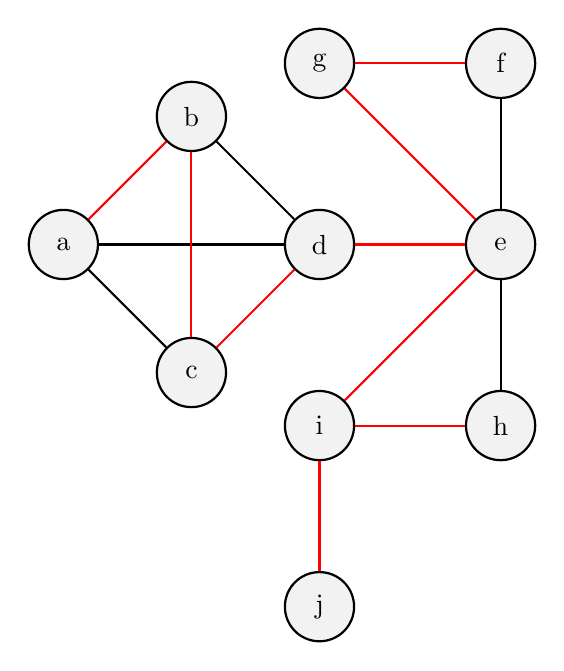
\begin{tikzpicture}[-,node distance=2.3cm,every state/.style={thick, fill=gray!10}, align=center]
        \node[state] (a) {a};
        \node[state,above right of=a] (b) {b};
        \node[state,below right of=b] (d) {d};
        \node[state,below right of=a] (c) {c};
        \node[state,right of=d] (e) {e};
        \node[state,above of=e] (f) {f};
        \node[state,left of=f] (g) {g};
        \node[state,below of=e] (h) {h};
        \node[state,left of=h] (i) {i};
        \node[state,below of=i] (j) {j};
        \draw
            (a) edge[color=red] node{} (b)
            (a) edge node{} (d)
            (a) edge node{} (c)
            (b) edge node{} (d)
            (b) edge[color=red] node{} (c)
            (c) edge[color=red] node{} (d)
            (d) edge[color=red] node{} (e)
            (e) edge[color=red] node{} (g)
            (f) edge[color=red] node{} (g)
            (e) edge node{} (f)
            (e) edge node{} (h)
            (e) edge[color=red] node{} (i)
            (i) edge[color=red] node{} (j)
            (i) edge[color=red] node{} (h)
            ;
    \end{tikzpicture}
    \end{subfigure}
    ~
    \begin{subfigure}{0.45\textwidth}
    \caption{Arestas e vértices de corte do grafo estão em destaque.}
    \label{fig:caso-teste1-resultado}
    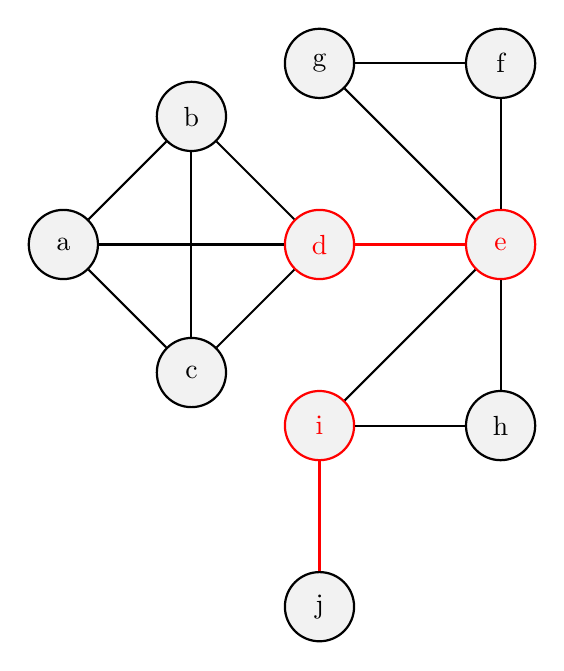
\begin{tikzpicture}[-,node distance=2.3cm,every state/.style={thick, fill=gray!10}, align=center]
        \node[state] (a) {a};
        \node[state,above right of=a] (b) {b};
        \node[color=red,state,below right of=b] (d) {d};
        \node[state,below right of=a] (c) {c};
        \node[color=red,state,right of=d] (e) {e};
        \node[state,above of=e] (f) {f};
        \node[state,left of=f] (g) {g};
        \node[state,below of=e] (h) {h};
        \node[color=red,state,left of=h] (i) {i};
        \node[state,below of=i] (j) {j};
        \draw
            (a) edge node{} (b)
            (a) edge node{} (d)
            (a) edge node{} (c)
            (b) edge node{} (d)
            (b) edge node{} (c)
            (c) edge node{} (d)
            (d) edge[color=red] node{} (e)
            (e) edge node{} (g)
            (f) edge node{} (g)
            (e) edge node{} (f)
            (e) edge node{} (h)
            (e) edge node{} (i)
            (i) edge[color=red] node{} (j)
            (i) edge node{} (h)
            ;
    \end{tikzpicture}
    \end{subfigure}
    \legend{Fonte: Próprio autor}
\end{figure*}

\begin{table*}[htb]
    \centering
    \caption{Tabela com a aplicação do algoritmo no grafo da \autoref{fig:caso-teste1}.}
    \begin{tabular}{c|c|c|c}
        \label{tab:caso1}
        Ancestral comum & Nó & Aresta de corte & Vértice de corte \\
        \hline
        a & b & - & - \\
        a & c & - & - \\
        a & d & - & - \\
        a & e & (d, e) & d, e \\
        e & f & - & - \\
        e & g & - & - \\
        e & h & - & - \\
        e & i & - & - \\
        e & i & (i, j) & i \\
        i & - & - & - \\
    \end{tabular}
\end{table*}

\begin{figure*}[htb]
    \centering
    \begin{subfigure}{0.45\textwidth}
    \caption{Grafo do segundo caso de testes.}
    \label{fig:caso-teste2}
    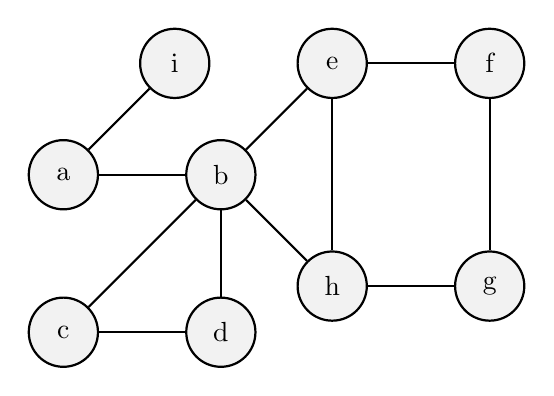
\begin{tikzpicture}[-,node distance=2cm,every state/.style={thick, fill=gray!10}, align=center]
        \node[state] (a) {a};
        \node[state,above right of=a] (i) {i};
        \node[state,right of=a] (b) {b};
        \node[state,below of=b] (d) {d};
        \node[state,left of=d] (c) {c};
        \node[state,above right of=b] (e) {e};
        \node[state,below right of=b] (h) {h};
        \node[state,right of=e] (f) {f};
        \node[state,right of=h] (g) {g};
        
        \draw
            (a) edge node{} (i)
            (a) edge node{} (b)
            (b) edge node{} (c)
            (b) edge node{} (d)
            (c) edge node{} (d)
            (b) edge node{} (e)
            (b) edge node{} (h)
            (e) edge node{} (f)
            (e) edge node{} (h)
            (h) edge node{} (g)
            (f) edge node{} (g)
            ;
    \end{tikzpicture}
    \end{subfigure}
    ~
    \begin{subfigure}{0.45\textwidth}
    \caption{Grafo após aplicação do BFS. As arestas em destaque formam a árvore BFS. }
    \label{fig:caso-teste2-bfs}
    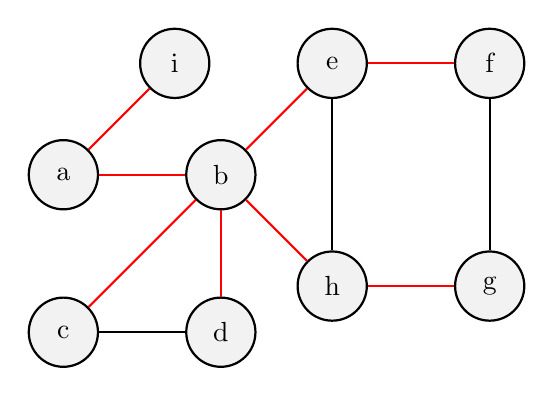
\begin{tikzpicture}[-,node distance=2cm,every state/.style={thick, fill=gray!10}, align=center]
        \node[state] (a) {a};
        \node[state,above right of=a] (i) {i};
        \node[state,right of=a] (b) {b};
        \node[state,below of=b] (d) {d};
        \node[state,left of=d] (c) {c};
        \node[state,above right of=b] (e) {e};
        \node[state,below right of=b] (h) {h};
        \node[state,right of=e] (f) {f};
        \node[state,right of=h] (g) {g};
        
        \draw
            (a) edge[color=red] node{} (i)
            (a) edge[color=red] node{} (b)
            (b) edge[color=red] node{} (c)
            (b) edge[color=red] node{} (d)
            (c) edge node{} (d)
            (b) edge[color=red] node{} (e)
            (b) edge[color=red] node{} (h)
            (e) edge[color=red] node{} (f)
            (e) edge node{} (h)
            (h) edge[color=red] node{} (g)
            (f) edge node{} (g)
            ;
    \end{tikzpicture}
    \end{subfigure}
    ~
    \begin{subfigure}{0.45\textwidth}
    \caption{Grafo após aplicação do DFS. As arestas em destaque formam a árvore DFS. }
    \label{fig:caso-teste2-dfs}
    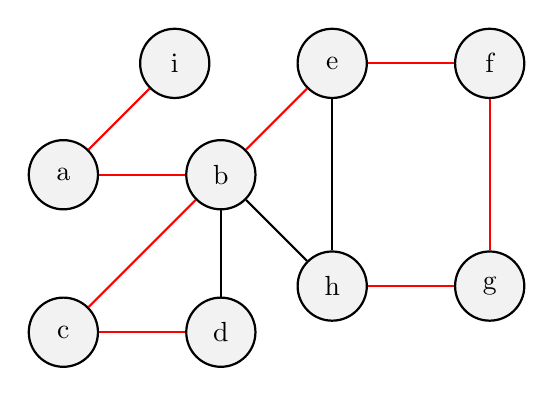
\begin{tikzpicture}[-,node distance=2cm,every state/.style={thick, fill=gray!10}, align=center]
        \node[state] (a) {a};
        \node[state,above right of=a] (i) {i};
        \node[state,right of=a] (b) {b};
        \node[state,below of=b] (d) {d};
        \node[state,left of=d] (c) {c};
        \node[state,above right of=b] (e) {e};
        \node[state,below right of=b] (h) {h};
        \node[state,right of=e] (f) {f};
        \node[state,right of=h] (g) {g};
        
        \draw
            (a) edge[color=red] node{} (i)
            (a) edge[color=red] node{} (b)
            (b) edge[color=red] node{} (c)
            (b) edge node{} (d)
            (c) edge[color=red] node{} (d)
            (b) edge[color=red] node{} (e)
            (b) edge node{} (h)
            (e) edge[color=red] node{} (f)
            (e) edge node{} (h)
            (h) edge[color=red] node{} (g)
            (f) edge[color=red] node{} (g)
            ;
    \end{tikzpicture}
    \end{subfigure}
    ~
    \begin{subfigure}{0.45\textwidth}
    \caption{Arestas e vértices de corte do grafo estão em destaque.}
    \label{fig:caso-teste2-resultado}
    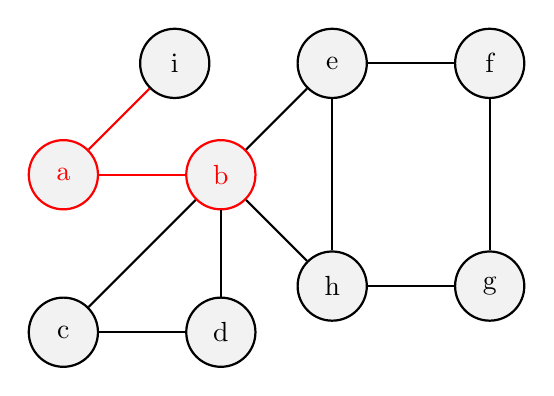
\begin{tikzpicture}[-,node distance=2cm,every state/.style={thick, fill=gray!10}, align=center]
        \node[color=red,state] (a) {a};
        \node[state,above right of=a] (i) {i};
        \node[color=red,state,right of=a] (b) {b};
        \node[state,below of=b] (d) {d};
        \node[state,left of=d] (c) {c};
        \node[state,above right of=b] (e) {e};
        \node[state,below right of=b] (h) {h};
        \node[state,right of=e] (f) {f};
        \node[state,right of=h] (g) {g};
        
        \draw
            (a) edge[color=red] node{} (i)
            (a) edge[color=red] node{} (b)
            (b) edge node{} (c)
            (b) edge node{} (d)
            (c) edge node{} (d)
            (b) edge node{} (e)
            (b) edge node{} (h)
            (e) edge node{} (f)
            (e) edge node{} (h)
            (h) edge node{} (g)
            (f) edge node{} (g)
            ;
    \end{tikzpicture}
    \end{subfigure}
    \legend{Fonte: Próprio autor}
\end{figure*}

\begin{table*}[htb]
    \centering
    \caption{Tabela com a aplicação do algoritmo no grafo da \autoref{fig:caso-teste2}.}
    \begin{tabular}{c|c|c|c}
        \label{tab:caso2}
        Ancestral comum & Nó & Aresta de corte & Vértice de corte \\
        \hline
        a & b & - & - \\
        a & i & - & a \\
        a & c & \textbf{(b, c)} & \textbf{b, c} \\
        c & d & \textbf{(c, d)} & \textbf{c, d} \\
        d & e & \textbf{(b, e)} & \textbf{b, e} \\
        e & f & - & - \\
        e & g & \textbf{(f, g)} & \textbf{f, g} \\
        g & h & \textbf{(g,h)} & \textbf{g, h} \\
        g & i & (a,i) & a \\
        
    \end{tabular}
\end{table*}

\begin{table*}[htb]
\centering
\caption{Resultados das execuções para os casos de testes e de validação.}
\begin{tabular}{c|c|c|c|c|c|c|c}
\label{tab:execucoes}
\multirow{2}{*}{Grafo} & \multicolumn{3}{c|}{Aresta de corte } & \multicolumn{3}{c|}{Vértice de corte } &   \\ 
\cline{2-7}
 & acertos & falso positivo & faltantes  & acertos & falso positivo & faltantes   &   \\ 
\cline{1-7}
Teste 1 & 2 & 0 & 0 & 3 & 0 & 0 \\
Teste 2 & 1 & 5 & 1 & 2 & 6 & 0 \\
aves-weaver-social & 2 & 28 & 3 & 5 & 29 & 0 \\
web-webbase-2001 & 5416 & 5054 & 4012 & 846 & 4489 & 1 \\
tech-WHOIS & 363 & 6869 & 79 & 254 & 6094 & 1 \\
drosophila-medulla & 318 & 1347 & 85 & 265 & 1075 & 1 \\
\end{tabular}
\end{table*}

\section{Trabalhos relacionados}
Os trabalhos foram selecionados mediante a uma revisão sistemática, afim de não enviesar a pesquisa. Todos os trabalhos têm como objetivo encontrar arestas e vértices de corte de um grafo e, é isto o que possuem em comum, mas cada um o faz com estratégias diferentes.

No artigo de \cite{italiano2012} são apresentados algoritmos de tempo linear para computar todas as arestas de corte e todos os vértices de corte de grafos direcionados explorando uma conexão entre vértices e arestas de corte.

Para encontrar as arestas de corte é escolhido um vértice qualquer para inicial, em seguida é determinado o conjunto de dominadores (vértices em que todos os caminhos para qualquer vértices passam por eles) de arestas, calculado o grafo reverso e determinado o conjunto de dominadores de arestas deste grafo reverso, por fim, a saída é a união do conjunto de dominadores de arestas e com a inversão das arestas do conjunto de dominadores de arestas do grafo reverso.

Para encontrar os pontos de articulação (vértices de corte), é escolhido arbitrariamente um vértice para testar se ele é um ponto de articulação, se for, a saída é este próprio vértice; é calculado o conjunto de dominadores não triviais de \textit{G(s)}, depois é determinado o grafo reverso e calculado o conjunto de dominadores não triviais neste grafo reverso e, por fim, a saída é a união dos dominadores de \textit{G(s)}  com os dominadores do $G^R(s)$.

No artigo de \cite{ibarra1993} é evidenciado que os pontos de articulação (vértice de corte) e pontes (aresta de corte) do grafo de permutação podem ser encontrados em $O (\log n)$, diferentemente do tradicional algoritmo de busca em profundidade que demora $O (\log n)$ com $O (n^2/\log n)$ processadores. Os algoritmos fazem permutações no grafo, para aproveitar as propriedades especiais de um grafo com permutação e, assim um meio mais eficiente para encontrar tais vértices e arestas de corte.

Sendo $\pi$ uma função de permutação e \textit{v} um vértice qualquer do grafo:
\begin{itemize}
\item se $\pi(v) < v$ o vértice \textit{v} é chamado de positivo;
\item se $\pi(v) = v$ o vértice \textit{v} é chamado de neutro;
\item se $\pi(v) > v$ o vértice \textit{v} é chamado de negativo.
\end{itemize}

Todo vértice não neutro pode ser um vértice de corte, então para ser um ponto de articulação, os itens devem ser atendidos:

\begin{enumerate}
\item Os nós \textit{i} e \textit{i-1} são iguais a 1;
\item existe um vértice \textit{u} < \textit{i} e que $\pi(u)=i$.
\end{enumerate}

Um outro fato que torna o algoritmo eficiente é a redução do conjunto de arestas que podem ser pontes não simples, com esta redução basta apenas focar nos pontos de articulação.

Além disso, esses algoritmos podem ser estendidos para resolver o problema dos componentes bi-conexos.

No artigo de \cite{madhumangal1998} é apresentado um algoritmo para encontrar todos os pontos de articulação (vértice de corte) de um grafo de permutação. O algoritmo proposto leva $O(n \log n)$ tempo e \textit{O(n)} espaço, onde n é o número de vértices.

O algoritmo não é tão trivial para uma explicação mais detalhada, mas a ideia é gerar um gráfico bidimensional (linhas verticais e horizontais) a partir dos vértices e, então os pontos de intersecção das linhas indicam um ponto de articulação, assim o problema é reduzido a encontrar o número \textit{i} da intersecção das linhas \textit{L(i)} e \textit{V(i)}; a Figura A mostra como fica este gráfico.


\begin{figure*}
\centering
\caption{Os vértices correspondentes às linhas pontilhadas são os pontos de articulação, são os vértices 2, 4 e 7 são pontos de articulação}
\includegraphics[width=\textwidth]{Figuras/verticesExample}
\end{figure*}

No artigo de \cite{henzinger2015} são expostos algoritmos para determinar os componentes fortemente conectados de 2-arestas e 2-vértices de um grafo direcionado. Uma explicação detalhada não é tão trivial de se fazer, mas de modo geral, a ideia é pegar um conjunto isolado de vértices de conectividade 2. Nos grafos não-dirigidos, os componentes conectados de 2 e 2 vértices podem ser encontrados em tempo linear.

\section{Considerações finais}
Uma das maiores dificuldades é que os artigos encontrados fazem demonstrações para provar a validade dos algoritmos elaborados, o que não é uma tarefa trivial de acompanhar ou explicar no presente artigo.

No tocante sobre o algoritmo, foi observado que ele só identifica arestas e vértices de corte em grafos que possuam ciclos triangulares, ciclos maiores que isso são problemáticos; na Tabela 2 as arestas e vértices de corte em destaque são os falso positivo, ou seja, pelo algoritmo são identificado como de corte quando na realidade não são. Portanto, esta solução fica limitada a grafos que possuam ciclos triangulares. Essa conclusão foi constatada observando as árvores que são geradas pelos algoritmos de buscas e como o algoritmo proposto atua nos grafos;  tendo resultado eficaz em grafos que contém ciclos com até três vértices.
\bibliography{bibliography}
\end{document}
